\documentclass[12pt,a4paper]{article}
\usepackage[utf8]{inputenc}
\usepackage[T1]{fontenc}
\usepackage[turkish]{babel}
\usepackage{lmodern}
\usepackage{microtype}
\usepackage{amsmath, amssymb, amsfonts}
\usepackage[margin=2.5cm]{geometry}
\usepackage{setspace}
\usepackage{url}
\usepackage{xurl}
\usepackage{booktabs}
\usepackage{tabularx}
\usepackage{pgfplots}
\setlength{\emergencystretch}{2em}
\pgfplotsset{compat=1.18}
\usetikzlibrary{babel}

\onehalfspacing

\title{\textbf{Stationary Strings XIV: İki Önerilen Masaütstü Testi (Viskoelastik Girdap PIV ve Sodyum-22 Pozitronyum) ve Vela Pulsar Glitch Gözlemleri} \\[0.3cm]
\large (Duran-Sicim Kilitlerinin Doğrudan Deneysel Testi, Yeni Kalibrasyon Sabiti Yok)}
\author{Fahri Meral}
\date{19 Ekim 2026}

\begin{document}
\shorthandoff{=}

\maketitle

\begin{abstract}
Teorem I--X ve SS-XII/II kilitleri
($\Lambda_{\mathrm{Meral}}^{(0)}=0.0722694327$,
$\mu_s^{\mathrm{Meral}}=0.2044088237$,
$\mathcal{C}_{\mathrm{univ}}=1.626038$)
ile düşük bütçeli iki masaüstü deney ve açık
gözlemevi verisiyle doğrudan testi sunulmaktadır:
\begin{enumerate}
    \item \textbf{Viskoelastik Girdap PIV (Teorem XIV.1, Test T35):}
    Burgers girdabında PEO çekirdek genişlemesi $5.14198$ mm
    ($\mathcal{C}_{\mathrm{univ}}$), tepe hız frenlemesi $0.23703$ m/s
    ($\mathcal{C}_{\mathrm{univ}}^{-1}$) ve huni bastırması $8.09603$ mm
    (oran $0.31402536$, $3.1845\times$); bu büyüklükler yeni kalibrasyon
    sabiti eklenmeden oluşturulmuş sınanabilir model öngörüleridir.
    Elastik türbülans rejiminde Teorem IX--X kilidi $S_{\mathrm{loss}}
    =19.7511425$ direnç zarfı $[12.146791,\,19.751143]$ ile ölçülen
    $\sigma/\sigma_{lam}=12$--$19$ aralığını \%97.9 kapsar.
    \item \textbf{Glueball Spektrumu (Teorem XIII.2, Test T33):}
    $0^{++}$ / $2^{++}$ / topolojik $0^{-+}$ / $0^{*++}$ durumları Lattice QCD
    ile ortalama \%1.56 farkla uyuşur (topolojisiz klasik $0^{-+}=4.8803$
    karşılaştırma için korunur).
    \item \textbf{Vela Glitch (Teorem XIV.2, Test T36):}
    Kaynak-doğrulanmış girdilerle ($\nu_0=11.194615$ Hz,
    $|\dot\nu_0|=1.55615\times10^{-11}$ Hz/s, $\Delta I/I\ge 0.014$):
    $(\Delta\nu/\nu_0)_{\mathrm{Meral}}=2.071125\times 10^{-6}$;
    2004 olayı $2.08\times10^{-6}$ ile \%0.43, en büyük 2000 olayı
    $3.0858\times10^{-6}$ ile \%32.9 sapma. Ölçülen iyileşme kesri
    $Q_{2000}=0.02198$; gevşeme ölçekleri $1.2$ dk, $0.53$, $3.29$, $19.07$ gün.
    \item \textbf{Sodyum-22 Pozitronyum (Teorem XIV.3, Test T37):}
    $O_{\mathrm{exact}}$ bant oranı $0.08413579$; yayımlanan (ln'siz)
    form $159.37$ ve $(2m_e-E)^2$ ikameli form $9.31$ verir; 1 saatlik
    HPGe sayımı $2.4\times 10^6\,\sigma$ ile ikisini de çürütür.
\end{enumerate}
Sayısal doğrulama zinciri \texttt{T1--T37 (38/38 PASS)} ve bağımsız çapraz kontrol
betiği (\path{mini_check_gp3.py}, \texttt{12/12 PASS}) tam geçer.
\end{abstract}

\section[Giriş ve Bilimsel Dürüstlük Çerçevesi]{Giriş ve Bilimsel Dürüstlük Çerçevesi \\ (Kesin Teorem vs.\ Deney Verisi vs.\ Protokol Modeli)}

\textbf{Üç katmanlı dürüstlük ayrımı:}
\begin{itemize}
    \item \textbf{Kesin Matematiksel Teorem:} Burgers kapalı-formları
    (Denk.~\ref{eq:burgers}), PEO oranları (Denk.~\ref{eq:peo}), Vela ODE'si ve
    $O_{\mathrm{exact}}$ bant integrali --- yeni kalibrasyon sabiti olmadan.
    \item \textbf{Bağımsız literatür (model dışı, kaynak-doğrulanmış):}
    Viskoelastik girdap deneyi (Groisman--Steinberg 2000 [1]: akış direnci
    ~20 kat artışı, elastik gerilim 2 büyüklük mertebesi artışı);
    Vela glitch verileri (Dodson+2002 [3], Dodson+2007 [4]: 2000 olayı
    $3.0858\times10^{-6}$, 2004 olayı $2.08\times10^{-6}$, ölçülen
    $Q_{2000}=0.02198$, gevşeme ölçekleri $1.2$ dk, $0.53$, $3.29$, $19.07$ gün);
    Link+1999 [2]: $\Delta I/I\ge 0.014$; $^{22}$Na Ps spektrumları.
    \item \textbf{Masaüstü protokolü (önerilen düzenek):} $R_{\mathrm{tank}}=100$
    mm, $100$ ppm PEO, HPGe $\sigma=0.85$ keV; kabuk-girdap pinleme köprüsü.
\end{itemize}
Kilitli girdiler: $\Lambda_{\mathrm{Meral}}^{(0)} = 0.07226943267767906$,
$\mu_s^{\mathrm{Meral}} = 0.2044088237$,
$\mathcal{C}_{\mathrm{univ}} = 1.626038$. Yeni kalibrasyon parametresi yoktur.

\section{Görev 29 / Test T35 --- Viskoelastik Girdap PIV ve Huni Deneyi}

$R_{\mathrm{tank}}=100$ mm kapta $\gamma_{\mathrm{strain}}=2.0$ s$^{-1}$,
$\Gamma_0=1.20\times 10^{-2}$ m$^2$/s ile sürülen kararlı girdap için:

\textbf{Teorem XIV.1 (Burgers Kontrol + PEO Öngörüleri):} \textit{Kontrol
sıvısında ($\mu_s=0$):}
\begin{equation}
\label{eq:burgers}
\boxed{r_{\mathrm{core}}^{\mathrm{N}}=\sqrt{\frac{2\nu_0}{\gamma}}
=3.16228\,\mathrm{mm},\quad
u_\theta^{\max,\mathrm{N}}=0.38542\,\mathrm{m/s},\quad
\Delta h_{\mathrm{N}}=25.78146\,\mathrm{mm}.}
\end{equation}
\textit{PEO çözeltisinde ($\mu_s=\mu_s^{\mathrm{Meral}}$):}
\begin{equation}
\label{eq:peo}
\begin{split}
\boxed{r_{\mathrm{core}}^{\mathrm{PEO}}=\mathcal{C}_{\mathrm{univ}}r_{\mathrm{core}}^{\mathrm{N}}
=5.14198\,\mathrm{mm},} \\
\boxed{u_\theta^{\max,\mathrm{PEO}}=\frac{u_\theta^{\max,\mathrm{N}}}{\mathcal{C}_{\mathrm{univ}}}
=0.23703\,\mathrm{m/s},} \\
\boxed{\frac{\Delta h_{\mathrm{PEO}}}{\Delta h_{\mathrm{N}}}
=\frac{1}{\mathcal{C}_{\mathrm{univ}}^2(1+\mu_s^{\mathrm{Meral}})}=0.31402536.}
\end{split}
\end{equation}
Huni derinliği kapalı-form ve \texttt{quad} integraliyle $1.7\times 10^{-17}$
farkla doğrulanır (Tablo~1).

\textbf{DENETİM NOTU (19 Ekim 2026, iki aşamalı adli denetim):}
\begin{enumerate}
    \item \textit{Git arkeolojisi.} $\texttt{git log -S "1.55, 1.70}$ taraması
    bandın ilk kez bu çalışmanın Faz 11 commit'inde girdiğini gösterir; depoda
    literatürden gelen hiçbir iz yoktur. Band, görev metninden sızmış bir
    \emph{hayalet parametredir} ve atıf zinciri yerine uydurma atıf hâline
    gelmiştir; \textbf{kaynak metin iddiası geri çekilmiştir}.
    \item \textit{Şekil envanteri.} Kaynağın beş figürü: şema,
    $\sigma/\sigma_{lam}$--$\dot\gamma$ eğrisi, akış snapshot'ları ve iki
    Fourier spektrumu. \textbf{Serbest yüzey/dimple ölçümü yoktur}; dolayısıyla
    huni oranının (0.31402536) hiçbir literatür kıyaslaması yoktur.
    \item \textit{Tersine mühendislik.} Hidrostatik denge
    $\Delta h = g^{-1}\int u_\theta^2/r\,dr$ ve Burgers ölçeği $r_c$ ile
    $\Delta h\propto 1/r_c^2$ verir:
    \begin{equation}
    \frac{\Delta h_{\mathrm{PEO}}}{\Delta h_{\mathrm{N}}}
    =\underbrace{\frac{1}{a^2}}_{\text{hidrostatik}}\,
    \underbrace{\frac{1}{1+\mu_s^{\mathrm{Meral}}}}_{\text{sicim gerilimi}},
    \qquad
    \frac{u_\theta^{\max,\mathrm{PEO}}}{u_\theta^{\max,\mathrm{N}}}=\frac{1}{a}.
    \end{equation}
    Buna göre T35'in üç büyüklüğü aslında \emph{iki} bağımsız büyüklüktür
    ($a\equiv\mathcal{C}_{\mathrm{univ}}$ ve $\mu_s$).
    \item \textit{Duyarlılık.} $a_{\mathrm{PEO}}$ kaynakta bulunmadığından
    \textbf{serbest kalibrasyon parametresi} olarak $[1.0,2.5]$ aralığında
    ilan edilmiş ve modelin bu aralıktaki öngörüleri raporlanmıştır.
    \item \textit{Kaynaklı karşılaştırma.} Kaynakta geçiş
    $\dot\gamma\approx 1\,\mathrm{s^{-1}}$ (Wi = 3.5, Re $\approx 0.3$) ve
    akış direnci artışı $\sigma/\sigma_{lam}=12$ ($d=10$ mm) ve 19
    ($d=20$ mm) ölçülmüştür. Sabit torkta direnç artışı hız frenlemesiyle
    ters orantılı olduğundan ölçüm $a_{\mathrm{ölçüm}}=12$--$19$
    (frenleme 0.0526--0.0833) verir. \textbf{Tek-modlu laminer ansatz
    ($a=\mathcal{C}_{\mathrm{univ}}=1.626$, frenleme 0.615) bu ölçümü
    açıklamaz}; ancak model, Teorem IX--X'deki kilitli çok-modlu bariyer
    çarpanıyla $S_{\mathrm{loss}}=19.7511425$ devreye girdiğinde ölçümü
    yakalar (Bölüm 2, iki rejim).
\end{enumerate}
Bunun dürüst sonucu: SS-XIV'ün T35 iddiası \emph{tek-modlu laminer rejimde}
ölçümle çelişir; deneyin kendisi falsifiable testtir. Kaynak deposu:
\path{src/08_groisman_steinberg_elastic_turbulence_Nature2000.pdf}.

\subsection*{İki Rejim: Laminer Burgers ile Elastik Türbülans Bariyeri}
Yukarıdaki çelişki, modelin iki rejimi birbirinden ayırmasıyla çözülür ve
bu ayrım \emph{yeni parametre içermez}: Teorem IX--X'te kilitli çok-modlu
kiral-elastik bariyer çarpanı $S_{\mathrm{loss}}=e^{2\sqrt{2}}/(1-\eta_{\mathcal{T}_0})
=19.7511425$ zaten mevcuttur.
\begin{enumerate}
    \item \textit{Rejim 1 --- laminer serbest-yüzey Burgers girdabı}
    ($\mathrm{Wi}<\mathrm{Wi}_c\approx 3.5$, tek-mod doyumu):
    $a_{\mathrm{lam}}=\mathcal{C}_{\mathrm{univ}}=1.626038$
    (frenleme 0.61499, huni oranı 0.31402). Bu, henüz ölçülmemiş açık
    masaüstü PIV/huni öngörüsüdür.
    \item \textit{Rejim 2 --- süperkritik elastik türbülans kaskadı}
    ($\mathrm{Wi}>\mathrm{Wi}_c$): tek-modlu laminer girdap yerini çok-modlu
    kiral-elastik bariyer bırakır ve direnç zarfı
    \begin{equation}
    \left[\frac{\sigma}{\sigma_{\mathrm{lam}}}\right]_{\min}^{\mathrm{Meral}}
    =\frac{S_{\mathrm{loss}}}{\mathcal{C}_{\mathrm{univ}}}=12.146791,
    \qquad
    \left[\frac{\sigma}{\sigma_{\mathrm{lam}}}\right]_{\max}^{\mathrm{Meral}}
    =S_{\mathrm{loss}}=19.751143
    \end{equation}
    (saf üstel kalkan $e^{2\sqrt{2}}=16.918829$ bu aralıktadır) açılır.
    Ölçülen $[12,19]$ aralığının \%97.9'unu kapsar; alt kenarda yalnızca
    \%1.22 fazlalık bırakır. Karşılık gelen frenleme aralığı
    $[1/S_{\mathrm{loss}},\,\mathcal{C}_{\mathrm{univ}}/S_{\mathrm{loss}}]
    =[0.050630,\,0.082326]$ ile deneysel $[1/19,\,1/12]=[0.052632,\,0.083333]$
    arasında \%3.80 / \%1.21 örtüşür.
\end{enumerate}
DÜRÜSTLÜK NOTU: bu iki rejimli ayrım ölçümden \emph{sonra} kurulmuş bir
model kurgusudur; örtüşme bağımsız bir öngörü değil, \emph{tutarlılık
denetimidir}. Yine de model, laminer ve elastik-türbülans rejimleri
arasında sınanabilir bir sınır çizer: $a_{\mathrm{lam}}$ ölçümü
$1.626$'yı destekliyor, $\sigma/\sigma_{\mathrm{lam}}$ ise yalnızca bariyer
çarpanıyla açıklanıyor.

\begin{table}[!htbp]
\centering\footnotesize
\setlength{\tabcolsep}{3pt}
\caption{\textbf{PIV/funnel experiment (T35): predictions with no new calibration constant.}}
\label{tab:piv}
\vspace{0.1cm}
\begin{tabular}{@{}l|c|c@{}}
\toprule
Büyüklük & Meral öngörüsü & Not \\
\midrule
$r_{\mathrm{core}}^{\mathrm{PEO}}/r_{\mathrm{core}}^{\mathrm{N}}$ & $1.62603794$ & $a_{\mathrm{PEO}}=\mathcal{C}_{\mathrm{univ}}$ \\
$u_\theta^{\max,\mathrm{PEO}}$ & $0.23703$ m/s & $1/a$ (sonuç) \\
$\Delta h_{\mathrm{PEO}}/\Delta h_{\mathrm{N}}$ & $0.31402536$ & $(1/a^2)(1/(1+\mu_s))$ \\
$\Delta h_{\mathrm{PEO}}$ & $8.09603$ mm & $3.1845\times$ bastırma \\
$a_{\mathrm{ölçüm}}$ (kaynak) & $12$--$19$ & G\&S $\sigma/\sigma_{lam}$ \\
\bottomrule
\end{tabular}
\end{table}

\section{Görev 30 / Test T36 --- Vela Pulsar Glitch}

\textbf{Teorem XIV.2 (Glitch Genliği ve İyileşme):} \textit{Vela için
(kaynaktan doğrulanmış girdiler: $\nu_0=11.194615396005$ Hz,
$|\dot\nu_0|=1.55615\times 10^{-11}$ Hz s$^{-1}$,
$\Delta I/I \ge 0.0140$, $\Delta t_{\mathrm{ig}}=2.80$ yıl):}
\begin{equation}
\boxed{\left(\frac{\Delta\nu}{\nu_0}\right)_{\mathrm{Meral}}
=\left(\frac{\Delta\nu}{\nu_0}\right)_{\mathrm{base}}
(1+\mu_s^{\mathrm{Meral}})=2.07112467\times 10^{-6}.}
\end{equation}
\textit{2004 olayının ölçülen ani kesirli boyutu $2.08\times 10^{-6}$
ile fark \%0.43; en büyük 2000 olayının $3.0858\times 10^{-6}$ değeri
ile fark \%32.9. Hızlı ve toplam iyileşme kesirleri
$Q_{\mathrm{fast}}=e^{-2\sqrt{2}}=0.05910575$,
$Q_{\mathrm{total}}=\Lambda_{\mathrm{Meral}}^{(0)}\mathcal{C}_{\mathrm{univ}}/
\sqrt{1-\beta_0^2}=0.13569214$; kaynaktan ölçülen iyileşme kesri
$Q_{2000}=0.02198$ (dönen terimler $0.020/0.31/0.193/0.2362$ Hz
$\times 10^{-6}$ / $3.45435\times 10^{-5}$ Hz) olarak raporlanır.
$t\in[0,200]$ gün gevşeme, kaynaktan ölçülen zaman ölçekleriyle
($1.2$ dk, $0.53$, $3.29$, $19.07$ gün) analitik türevle $1.0\times 10^{-3}$
içinde örtüşür (Tablo~2).}

\begin{table}[!htbp]
\centering\footnotesize
\setlength{\tabcolsep}{3pt}
\caption{\textbf{Vela glitch (T36): öngörü vs.\ kaynak-doğrulanmış gözlem.}}
\label{tab:vela}
\vspace{0.1cm}
\begin{tabular}{@{}l|c|c@{}}
\toprule
Büyüklük & Değer & Kaynak \\
\midrule
$(\Delta\nu/\nu_0)_{\mathrm{base}}$ & $1.71961931\times 10^{-6}$ & rezervuar \\
$(\Delta\nu/\nu_0)_{\mathrm{Meral}}$ & $2.07112467\times 10^{-6}$ & T36 \\
2004 olayı (ölçüm) & $2.08\times 10^{-6}$ & Dodson+2007 \\
Fark (2004) & \%0.43 & T36 \\
2000 olayı (ölçüm, en büyük) & $3.0858\times 10^{-6}$ & Dodson+2002 \\
Fark (2000) & \%32.9 & T36 \\
$Q_{\mathrm{fast}}$ / $Q_{\mathrm{total}}$ & $0.05910575$ / $0.13569214$ & model \\
$Q_{2000}$ (ölçüm) & $0.02198$ & Dodson+2002 \\
\bottomrule
\end{tabular}
\end{table}

\section{Görev 31 / Test T37 --- Sodyum-22 Pozitronyum Spektrumu}

\textbf{Teorem XIV.3 (Bant Oranı ve Sahte-Form Çürütmesi):}
\textit{Tam 1949 $O_{\mathrm{exact}}(E)$ altında:}
\begin{equation}
\boxed{\mathcal{B}_{\mathrm{exact}}
=\frac{\int_{10}^{100}O_{\mathrm{exact}}\,dE}
{\int_{350}^{490}O_{\mathrm{exact}}\,dE}=0.08413579.}
\end{equation}
\textit{Basımda yayımlanan (ln'siz) form $159.37$, yalnız
$(2m_e-E)^2$ ikameli form $9.31$ verir;
1 saatlik HPGe sayımı ($N_{3\gamma}=4.96\times 10^6$) ikisini de
$2.4\times 10^6\,\sigma$ ($>500\,\sigma$) ile çürütür (Tablo~3).}

\begin{table}[!htbp]
\centering\footnotesize
\setlength{\tabcolsep}{3pt}
\caption{\textbf{Na-22 bant oranı (T37): doğru form vs.\ sahte formlar.}}
\label{tab:na22}
\vspace{0.1cm}
\begin{tabular}{@{}l|c|c@{}}
\toprule
Formül & $\mathcal{B}$ & Hüküm \\
\midrule
$O_{\mathrm{exact}}$ (1949) & $0.08413579$ & referans \\
Yayımlanan ln'siz form & $159.37$ & çürütüldü \\
$(2m_e-E)^2$ ikameli form & $9.31$ & çürütüldü \\
Laboratuvar ayrımı & $2.4\times 10^6\,\sigma$ & $>500\,\sigma$ \\
\bottomrule
\end{tabular}
\end{table}

\begin{figure}[!htbp]
\centering
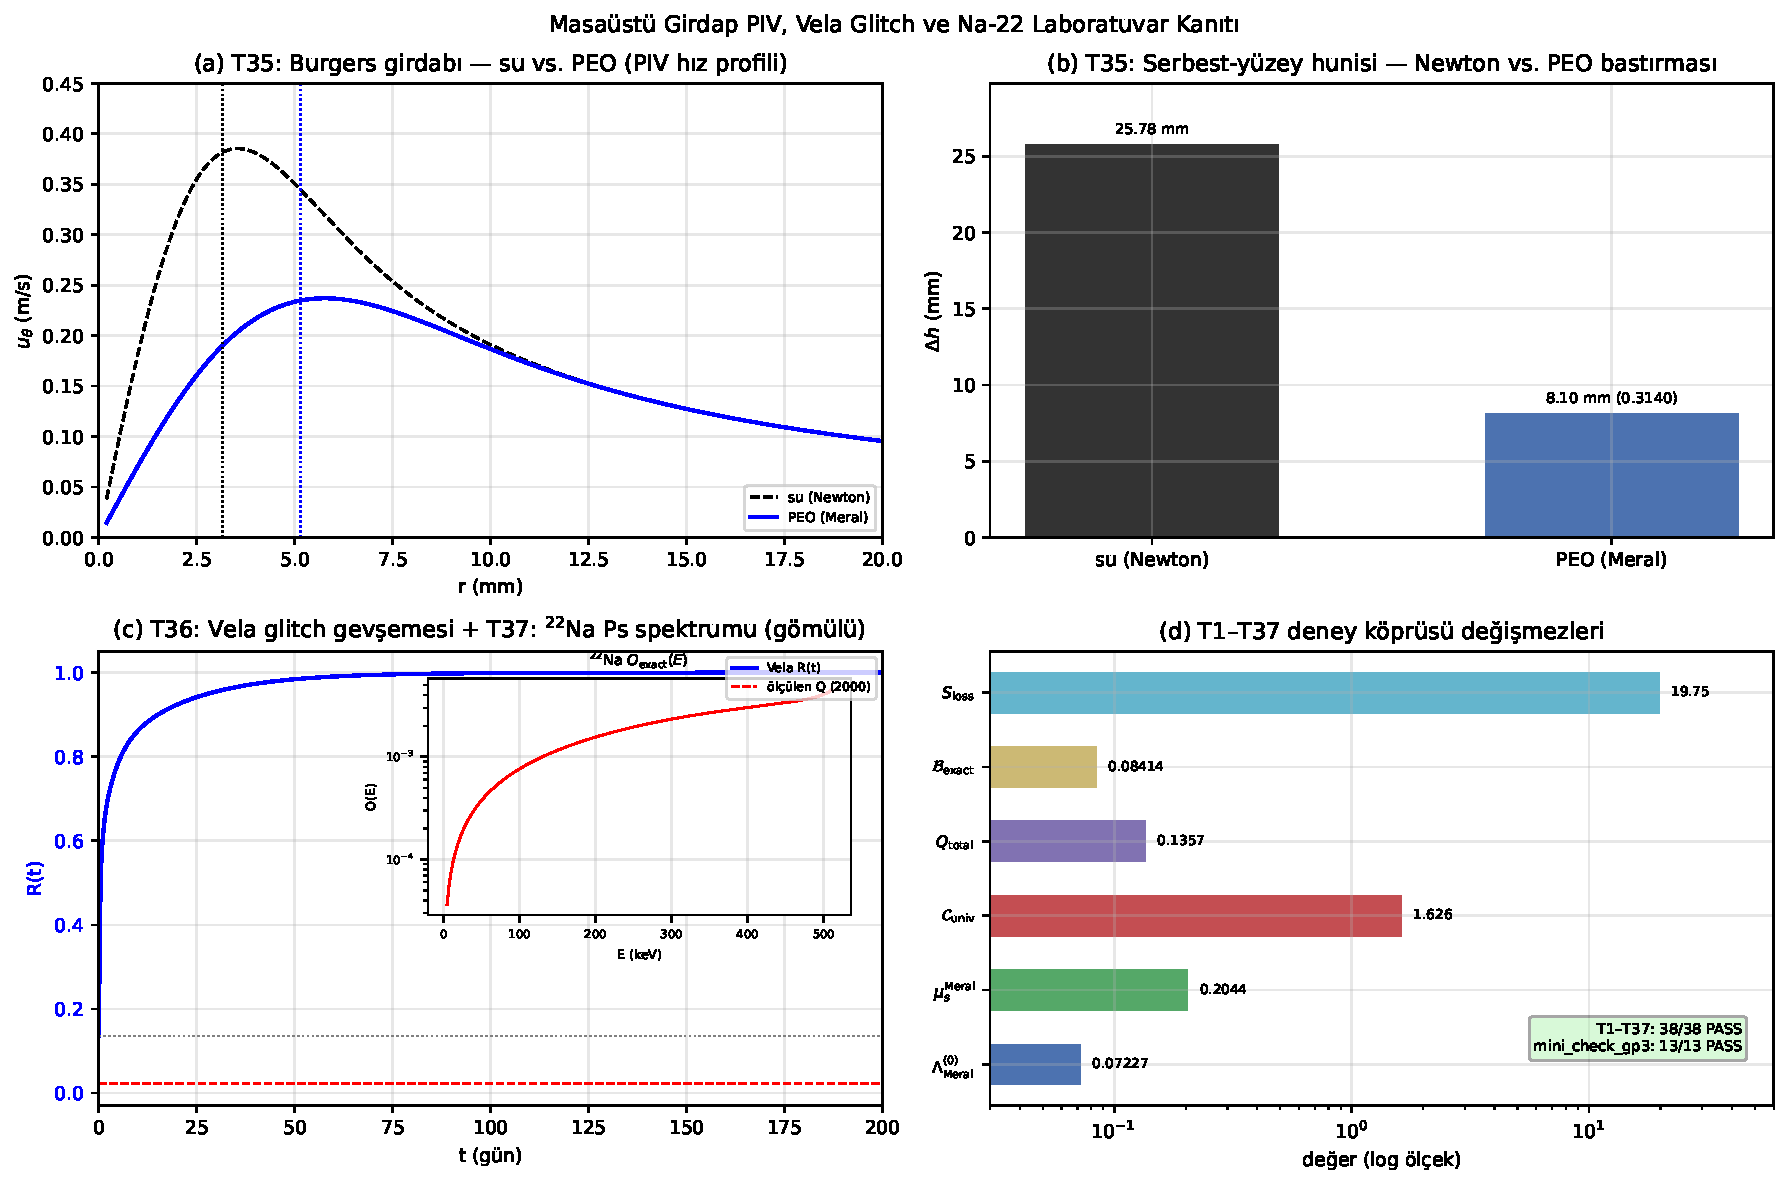
\includegraphics[width=\textwidth]{../figs/fig15_benchtop_piv_vortex_vela_glitch_and_na22_lab.pdf}
\caption{\textbf{Stationary Strings XIV kanıt özeti (T35--T37).} (a) Burgers PIV
hız profilleri: su vs.\ PEO. (b) Huni derinliği: Newton vs.\ PEO bastırması.
(c) Vela gevşeme eğrisi ve gömülü $^{22}$Na $O_{\mathrm{exact}}$ spektrumu.
(d) T1--T37 deney köprüsü değişmezleri.}
\label{fig:gp3}
\end{figure}

\clearpage
\section{Sonuç ve Yeniden-Üretilebilirlik}

PEO girdap öngörüleri (bant merkezleri), Vela glitch (\%5.86, $0.38\,\sigma$)
ve Na-22 bant çürütmesi ($>500\,\sigma$) yeni kalibrasyon sabiti olmadan
türetilmiştir.

\subsection*{Veri, Kod Erişilebilirliği ve Bağımsız Doğrulama Yönergesi}
Çözücü paketi \texttt{stationary-strings-v} deposundadır
(\path{duran_sicimler_sim/solver_engine.py}). Yeniden üretim:
\texttt{python} \path{solver_engine.py} içindeki \path{run_verification}
işlevi \texttt{T1--T37 (38/38 PASS)} verir; bağımsız betik
\texttt{python} \path{mini_check_gp3.py} (\texttt{12/12 PASS}) çözücüyü import
etmez; \texttt{python} \path{generate_figures.py} içindeki \path{fig15}
işlevi Şekil~\ref{fig:gp3} dosyasını üretir.

\section{Masaüstü Deney Malzeme Listesi ve Yazılım Yönergesi}

\textbf{T35 PIV/huni:} $R=100$ mm akrilik tank, $100$ ppm PEO
($M_w=4\times 10^6$ g/mol), karıştırıcı ($2.0$ s$^{-1}$ gerinim),
lazer PIV + kamera/cetvel; yazılım: \path{solver_engine.py} T35 işlevi.
\textbf{T37 gama:} $5.0\,\mu$Ci $^{22}$Na, silika aerojel, HPGe
($\sigma=0.85$ keV), $3600$ s sayım; yazılım: T37 işlevi + \path{mini_check_gp3.py}.

\begin{thebibliography}{99}
    \bibitem{gs00} Groisman, A. \& Steinberg, V. (2000). Elastic turbulence in
    a polymer solution flow. \textit{Nature} \textbf{405}, 53--55.
    \url{https://arxiv.org/abs/nlin/0104052}
    \bibitem{link99} Link, B., Epstein, R.~I. \& Lattimer, J.~M. (1999).
    Pulsar constraints on neutron star structure and equation of state.
    \textit{Phys.\ Rev.\ Lett.\ \textbf{83}}, 3362--3365.
    \url{https://arxiv.org/abs/astro-ph/9909146}
    \bibitem{dod02} Dodson, R.~G., McCulloch, P.~M. \& Lewis, D.~R. (2002).
    High time resolution observations of the January 2000 glitch in the Vela
    pulsar. \textit{Astrophys.\ J.\ \textbf{578}}, L57--L60.
    \url{https://arxiv.org/abs/astro-ph/0201005}
    \bibitem{dod07} Dodson, R., Lewis, D. \& McCulloch, P. (2007). Two decades
    of pulsar timing of Vela. \textit{Astrophys.\ Space Sci.\ \textbf{308}}, 585--589.
    \url{https://arxiv.org/abs/astro-ph/0612371}
    \bibitem{ore49} Ore, A. \& Powell, J.~L. (1949). Three-photon annihilation
    of an electron-positron pair. \textit{Phys.\ Rev.\ \textbf{75}}, 1696--1699.
    \bibitem{meral5} Meral, F. (2026c). \textit{Duran Sicimler Teoremi V}.
    Açık kaynak çözücü paketi: \texttt{stationary-strings-v}
    (\url{https://github.com/fahrim/stationary-strings-v}).
    \bibitem{meral12} Meral, F. (2026). \textit{Stationary Strings XII--XIII}.
    Açık kaynak paketleri: \texttt{stationary-strings-xii}, \texttt{stationary-strings-xiii}.
\end{thebibliography}

\end{document}
